\chapter{Svolgimento dello \textit{stage}}
\label{chap:svolgimento-stage}
\noindent
In questo capitolo descriverò in dettaglio lo svolgimento dello \textit{stage}, suddiviso nelle varie fasi che hanno caratterizzato il progetto.\\
Inizierò con la descrizione dell'analisi dei requisiti, dove verranno illustrate le esigenze e le aspettative degli \textit{stakeholder} e come queste sono state raccolte e documentate tramite le \textit{user story}.\\
Successivamente tratterò delle fasi di progettazione e codifica, spiegando le scelte architetturali e le tecnologie utilizzate per sviluppare il progetto.\\
Concluderò con la verifica, validazione e illustrando i risultati che ho ottenuto, sia da un punto di vista qualitativo che quantitativo.
% Ogni sezione fornirà una panoramica delle attività svolte, delle metodologie utilizzate e dei risultati ottenuti, con l'obiettivo di fornire una visione completa e dettagliata del lavoro svolto durante il periodo di \textit{stage}.

\section{Analisi dei requisiti}\label{sec:analysis}\noindent
% \texttt{Descrizione dell'attività di analisi dei requisiti.}
Per garantire che il prodotto finale soddisfi le aspettative e gli obiettivi, è necessario analizzare a fondo le varie esigenze e aspettative degli \textit{stakeholder} che esso dovrà soddisfare.
Per fare ciò, ho utilizzato l'approccio delle \textit{user story}, ovvero varie descrizioni semplici delle funzionalità dal punto di vista dell'utente.\\
Le \textit{user story} vengono raccolte e identificate in una lista tramite un codice, esso è strutturato nel seguente modo:
\begin{center}
    \textbf{US-[Numero incrementale]}
\end{center}\noindent
Queste \textit{user story} sono state approvate con il \textit{tutor} e ognuna di essa è mandatoria.
% Technically the code shoud use US and not just U
\begin{center}
    \rowcolors{1}{}{tableGray}
    \begin{longtable}{|p{2.5cm}|p{10.5cm}|}
    \hline
    \multicolumn{1}{|c|}{\textbf{Identificatore}} & \multicolumn{1}{c|}{\textbf{\textit{User story}}}\\ 
    \hline 
    \endfirsthead
    \rowcolor{white}
    \multicolumn{2}{c}{{\bfseries \tablename\ \thetable{} -- Continuo della tabella}}\\
    \hline
    \multicolumn{1}{|c|}{\textbf{Identificatore}} & \multicolumn{1}{c|}{\textbf{\textit{User story}}}\\ \hline 
    \endhead
    \hline
    \rowcolor{white}
    \multicolumn{2}{|r|}{{Continua nella prossima pagina...}}\\
    \hline
    \endfoot
    \endlastfoot
    
    \multicolumn{1}{|c|}{US-1} & Come utente, voglio che il \textit{dataset} pubblico PTB-XL venga usato per svolgere addestramenti di reti neurali artificiali, così che io possa provare diverse strutture nell'ambito dell'analisi di segnali elettrocardiografici. \\
    \hline
    \multicolumn{1}{|c|}{US-2} & Come utente, voglio che il \textit{dataset} venga caricato nella fase di \textit{training} senza sforare i limiti della RAM, in modo da permettere addestramenti di reti neurali artificiali con \textit{dataset} di qualsiasi dimensioni \\
    \hline
    \multicolumn{1}{|c|}{US-3} & Come utente, voglio che i parametri per l'addestramento di reti siano in un singolo posto, in modo da facilitare il processo di addestramento di nuovi modelli basati su nuove strutture \\
    \hline
    \multicolumn{1}{|c|}{US-4} & Come utente, voglio che la rete neurale artificiale abbia come come input aggiuntivo, oltre al segnale elettrocardiografico, anche altre informazioni come età e peso del paziente, in modo da aumentare i risultati dei modelli creati con i vari addestramenti \\
    \hline
    \multicolumn{1}{|c|}{US-5} & Come utente, voglio che ci sia la possibilità di fare \textit{preprocessing}, in modo da applicare funzioni per estrarre \textit{features} \\
    \hline
    % \multicolumn{1}{|c|}{US-6} & Come utente, voglio che ci sia la possibilità di applicare \textit{downsampling}, in modo da ridurre la dimensione dei dati in entrata \\
    % \hline
    % \multicolumn{1}{|c|}{US-7} & Come utente, voglio che i modelli addestrati diano in output due classi, in modo da capire se il paziente è sano o no \\
    % \hline
    % \multicolumn{1}{|c|}{US-8} & Come utente, voglio che i modelli addestrati diano in output cinque classi, in modo da capire in quale delle superclassi del \textit{dataset} fa parte la diagnosi dell'elettrocardiogramma \\
    % \hline
    % \multicolumn{1}{|c|}{US-9} & Come utente, voglio che i modelli addestrati possano essere confrontati con i \textit{file} del dataset privato, in modo da mantenere una compatibilità tra i due \textit{dataset} \\
    % \hline
    % \multicolumn{1}{|c|}{US-10} & Come utente, voglio che il programma crei una \gls{confusionmatrix}, in modo da valutare oggettivamente la prestazione del modello addestrato \\
    % \hline
    \multicolumn{1}{|c|}{...} & \multicolumn{1}{|c|}{...}  \\
    \hline
    \multicolumn{1}{|c|}{US-19} & Come utente, voglio che il programma crei un grafico di \gls{confidence} usando i dati del \textit{dataset} privato, in modo da valutare oggettivamente la prestazione del modello addestrato \\
    \hline
    \multicolumn{1}{|c|}{US-20} & Come utente, voglio che l'applicazione salvi ogni metrica e modelli creati in una \textit{directory} dedicata, in modo da poter salvare ogni addestramento svolto e dare la possibilità di confrontare i risultati se ce ne fosse bisogno \\
    \hline
    \hiderowcolors
    \caption{Tabella contenente le varie \textit{user story}.}
    \label{tab:user-stories}
    \end{longtable}
\end{center}

\section{Progettazione}\label{sec:design}\noindent
% \texttt{Descrizione dell'attività di progettazione.}

\subsection{Visione d'insieme}
\begin{figure}[H]
    \centering
    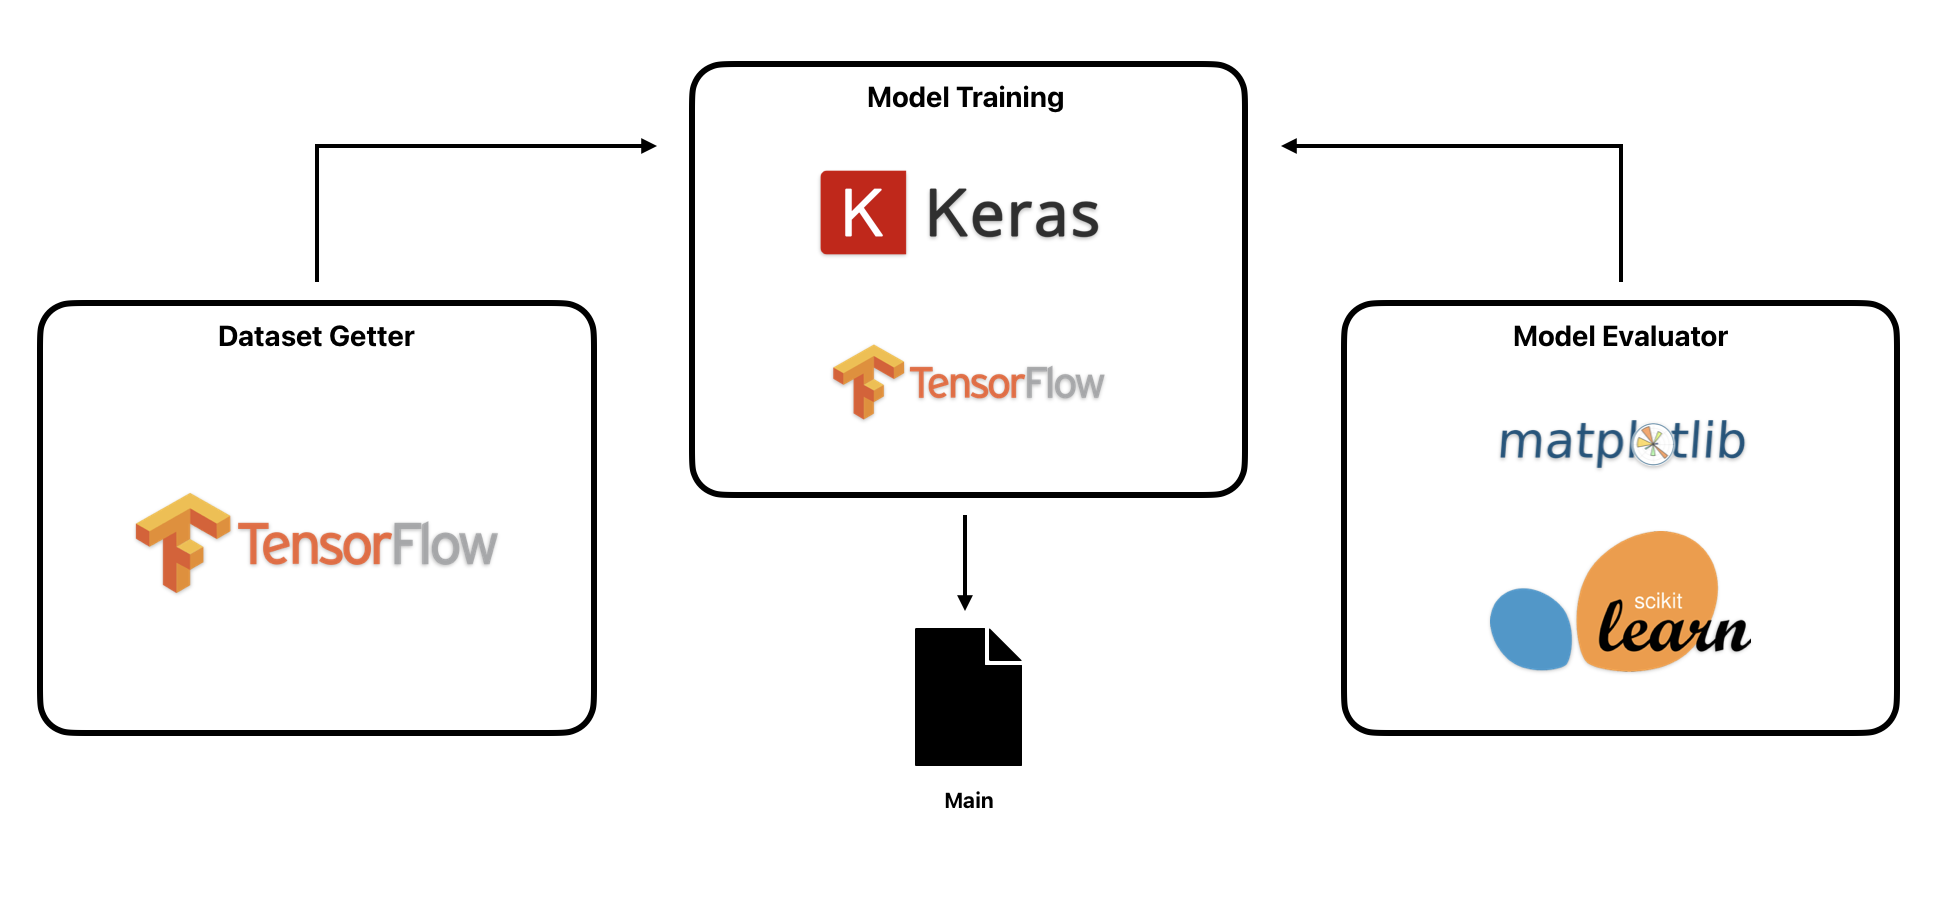
\includegraphics[alt={Architettura generale con le principali tecnologie utilizzate}, width=0.9\columnwidth]{img/design.png}
    \caption{\centering Architettura generale con le principali tecnologie utilizzate}
    \label{fig:desc-proj}
\end{figure}\noindent
L'applicazione progettata la si può vedere in tre macro sezioni, dove la principale di esse è quella che si occupa di effettuare l'addestramento delle reti neurali artificiali.\\
Per soddisfare i requisiti ho deciso di realizzare un semplice programma in Python utilizzabile dal terminale, quindi senza nessuna interfaccia grafica.
Questa scelta è dovuta sia dal fatto che non era richiesto per i requisiti, che dal fatto che non è necessario semplificare troppo l'utilizzo del programma, siccome ci si aspetta che l'utente finale sia già esperto e che voglia una certa libertà nella modifica dei parametri che vuole cambiare.\\
Ho deciso di progettare il programma incentrando tutto sul componente dedicato a svolgere gli addestramenti. Questo componente possiede due dipendenze, che sono: il componente dedicato all'ottenimento dei dati e il componente che si occupa di valutare il risultato.

\subsection{Addestramento di modelli}\noindent
Il \textit{focus} principale del programma è di creare modelli tramite l'addestramento di reti neurali artificiali. Per fare ciò ho utilizzato, come tecnologia principale, Keras.\\
Attraverso questa tecnologia è possibile creare modelli attraverso due API che sono disponibili all'utilizzo. Il loro funzionamento non è dissimile, ma possiedono delle caratteristiche fondamentali da capire:
\begin{itemize}
    \item \textbf{\textit{Sequential} API:} attraverso questa API la definizione dei modelli è veramente molto semplice, e risulta molto semplice anche il loro utilizzo. Però questa semplicità avviene ad un costo: ovvero che non è possibile inserire più \textit{input} di diverso tipo in contemporanea. Questo perchè i modelli che si possono definire, sono sequenziali e perciò sono una singola catena di processamento.
    \item \textbf{\textit{Functional} API:} attraverso questa API si possono definire modelli più complessi, ma anche l'utilizzo e definizione diventano relativamente più complessi. Questa intricatezza permette di creare modelli che supportano \textit{multi-input}, \textit{multi-output} oppure entrambi. 
\end{itemize}
\begin{figure}[H]
    \centering
    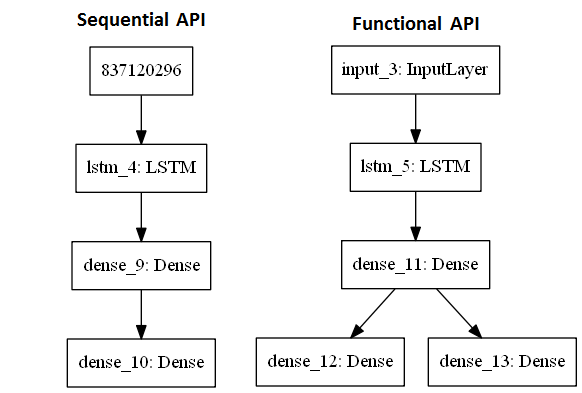
\includegraphics[alt={Confronto tra \textit{Sequential} API e \textit{Functional} API}, width=0.8\columnwidth]{img/seq-fun.png}
    \caption[Confronto tra \textit{Sequential} API e \textit{Functional} API]{\centering Confronto tra \textit{Sequential} API e \textit{Functional} API \par \textbf{Fonte:} \href{https://stackoverflow.com/questions/58092176/keras-sequential-vs-functional-api-for-multi-task-learning-neural-network}{stackoverflow.org}}
    \label{fig:desc-proj}
\end{figure}\noindent
Il programma da me progettato, include entrambe le API. L'utilizzo di una di esse viene deciso dall'utente nel \textit{file} principale di esecuzione del programma.\\
La scelta di implementare entrambe deriva dal fatto che l'utente finale necessita di confrontare l'influenza delle informazioni aggiuntive che vengono inserite nel modello sulle prestazioni finali ottenute. In questo specifico ambito, non è detto che informazioni aggiuntive come l'età e il peso del paziente influiscano notevolmente sulle prestazioni del modello creato.\\
Da un punto di vista teorico, le informazioni aggiuntive influiscono in modo positivo sulle prestazioni, però questa aggiunta espande il modello, e facendo ciò, vengono incrementati anche i requisiti prestazionali della macchina che deve eseguirlo.\\
Perciò ho deciso di implementare le due API sotto forma di due classi che implementano la stessa classe astratta, in modo da avere in comune più codice possibile.
\begin{figure}[H]
    \centering
    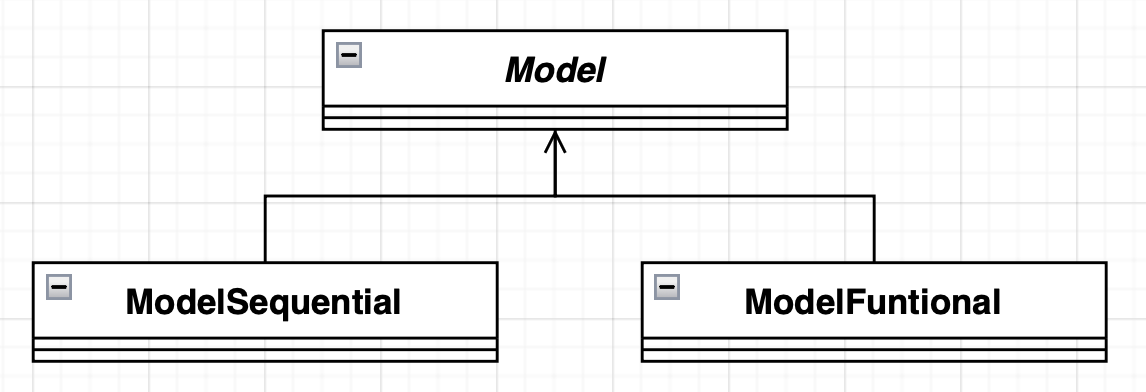
\includegraphics[alt={Diagramma delle classi di addestramento di reti neurali artificiali}, width=0.75\columnwidth]{img/model-diag.png}
    \caption{\centering Diagramma delle classi di addestramento di reti neurali artificiali}
    \label{fig:datasetgetter-diagram}
\end{figure}

\subsection{Gestione del \textit{dataset}}\noindent
Una delle dipendenze della parte di addestramento dei modelli è l'ottenimento dei dati su cui eseguire l'addestramento. Questo è un'importante passo negli addestramenti di reti neurali artificiali, senza di esso non sarebbe possibile neanche realizzare un singolo modello.\\
Per far sì che un addestramento avvenga, è necessario che i dati richiesti dall'addestramento stesso, siano disponibili all'interno della RAM, ma per fare ciò, ci sono due metodi:

\newpage

\begin{itemize}
    \item \textbf{Caricare l'intero \textit{dataset}:} questa è l'opzione più semplice da realizzare. Ha il vantaggio di predisporre tutti i dati necessari in una memoria veloce come la RAM, permettendo tempi di risposta tra le varie \glslink{epoch}{epoche} veramente bassi. Tuttavia, questo metodo viene utilizzato solo quando il \textit{dataset} utilizzato non è tanto grande, siccome più grande un \textit{dataset} è, più RAM è richiesta.
    \item \textbf{Caricare in modo dinamico:} questa opzione risolve il problema del limite della RAM. I file richiesti durante l'addestramento vengono letti dalla memoria per l'archiviazione a lungo termine quando sono necessari, o se si utilizza il \gls{prefetch}, momenti prima. Perciò i dati permangono per poco tempo all'interno della RAM prima di essere rimpiazzati dai dati successivi. Questo permette di utilizzare \textit{dataset} di qualsiasi dimensione per addestrare reti neurali artificiali in qualsiasi macchina si voglia. Lo svantaggio di questa tecnica è che è subisce un \textit{bottleneck} nel caso si sta addestrando un modello computazionalmente semplice. Questo per via del limite fisico dovuto alla lettura dei dati dalla memoria di archiviazione a lungo termine.
\end{itemize}
Questo progetto, come spiegato precedentemente, tratta di \textit{dataset} di grandi dimensioni, perciò posso considerare di sviluppare solo la seconda delle due opzioni qui sopra presentate.\\
Per implementare ciò, ho scelto di utilizzare i \textit{generator} disponibili utilizzando TensorFlow, essendo completamente compatibile con l'addestramento effetuato con Keras. Ero però dubbioso in che formato era meglio mantenere il \textit{dataset} per ottenere i migliori risultati di velocità nel caricamento dei dati.\\
Per capire ciò, ho sperimentato utilizzando diversi formati di file per cercare di ottenere il miglior compromesso tra dinamicità e velocità.\\
Prima di esporre quale soluzione ho deciso di utilizzare alla fine, vado ad esporre una delle soluzioni che ho sperimentato.
Essa era stata ideata basandosi sulla riduzione dei tempi di caricamento dei vari file, riducendo il numero di file da caricare.
Per fare ciò ho compresso i \textit{file} originali del \textit{dataset}, in vari file HDF5, un formato di \textit{file} progettato per la memorizzazione di grandi quantità di dati, in modo da avere un numero minore di \textit{file} con una dimensione leggermente più grande.
Questo ha permesso di avere tempi di risposta minori tra una epoca e l'altra nella fase di addestramento.
Ma è anche vero che questa soluzione possedeva due problemi:
\begin{itemize}
    \item \textbf{Gestione delle \gls{label}:} questa soluzione complicava la gestione delle etichette associate ai dati, che erano ora in gruppi di \textit{file}. Una possibile soluzione avrebbe portato a progettare un sistema più complicato del necessario, e avrebbe portato via molto tempo.
    \item \textbf{Troppa specificità:} decidere quanti dati inserire in un HDF5 \textit{file} è di per sè un dilemma. La dimensione di certi \textit{file} potrebbe andare bene per uno scenario d'installazione e d'uso, ma non è detto che sia la scelta più ottimale per altri scenari. Inoltre il vantaggio viene perso se si svolge addestramenti di modelli computazionalmente demandanti.
\end{itemize}
Perciò, considerando tutte le opzioni, ho deciso che era meglio mantenere i vari dati del \textit{dataset} nel loro formato originale. Per il semplice fatto che questa soluzione avrebbe portato alla minore produzione di codice, che è importante da considerare, siccome richiede meno modifiche in futuro, nel caso ce ne fosse bisogno.\\
Ho progettato questo componente similmente al componente precedentemente esposto: ovvero tramite una classe astratta da dove vengono implementate diverse classi concrete.
In questo caso, avere la classe astratta è di maggiore importanza. Questo perchè oltre a creare le due classi per dare l'\textit{input} alle due API, che ne richiedono due diversi, dovevo implementare anche un generatore per i \textit{file} \gls{dicom} che facevano parte del piccolo \textit{dataset} privato.
Questi \textit{file} sono una piccolissima frazione del \textit{dataset} con cui l'azienda si troverà a lavorare in futuro, perciò come da requisiti, dovevo implementarli per validare la possibilità di utilizzarli nel codice da me prodotto.
\begin{figure}[H]
    \centering
    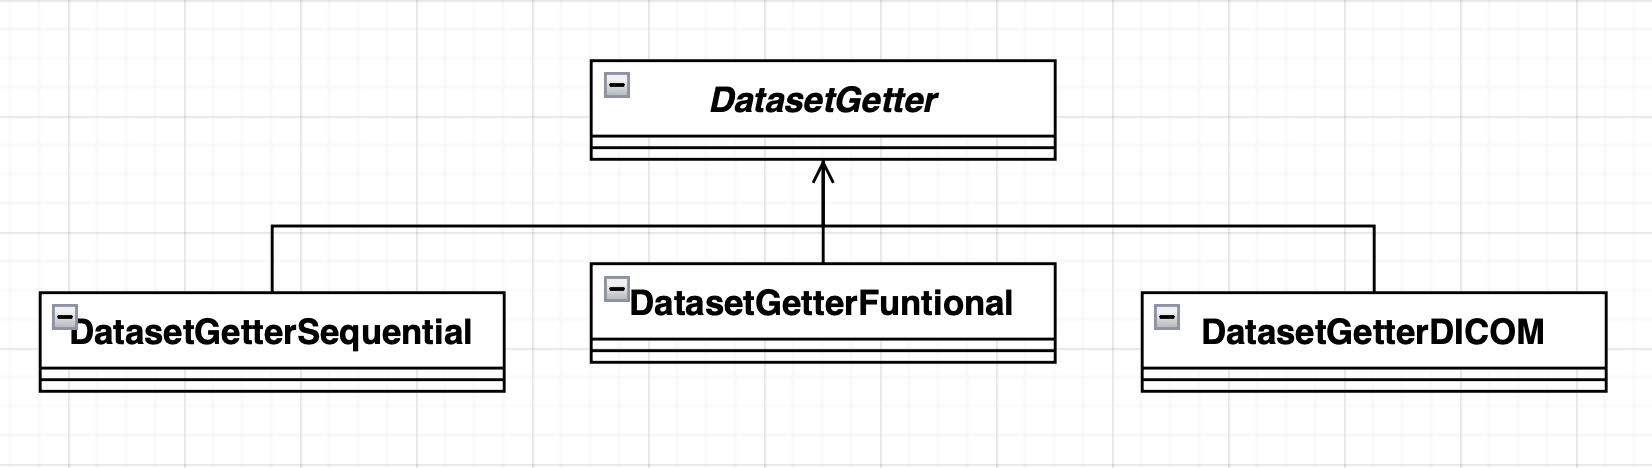
\includegraphics[alt={Diagramma delle classi di gestione del \textit{dataset}}, width=0.9\columnwidth]{img/dg-diag.png}
    \caption{\centering Diagramma delle classi di gestione del \textit{dataset}}
    \label{fig:datasetgetter-diagram}
\end{figure}

\subsection{Valutazione dei modelli}\noindent
L'ultima dipendenza per l'addestramento delle reti neurali artificiali è la realizzazione di vari \textit{output} che danno la possibilità di valutare oggettivamente le prestazioni del modello creato.\\
A fine dell'addestramento, il componente a esso dedicato si occupa di chiamare questo componente, che ricevendo determinate informazioni dell'addestramento, si occupa di generare le varie metriche richieste dai requisiti.
Di seguito vado ad esporre le metriche implementate:
\begin{itemize}
    \item \textbf{Grafici di andamento del \textit{training}:} durante l'addestramento, Keras, si occupa di valutare l'andamento. Prendendo le informazioni collezionate da Keras, è possibile creare dei grafici, utili per valutare varie cose.
    \item \textbf{\glslink{confusionmatrix}{Matrice di confusione}:} ``strumento'' utilizzato per comparare le predizioni di \textit{test} che un modello svolge, con gli effettivi risultati.
    \item \textbf{\glslink{confidence}{Confidenza}:} generalmente un'istogramma dove viene visualizzata l'incertezza del modello nelle predizioni che svolge durante la fase di \textit{test}.
    \item \textbf{Varie statistiche:} si tratta di una lista di metriche in forma testuale, che valuta numericamente le prestazioni del modello nel predirre. Una delle metriche più notevoli è quella dell'accuratezza, che indica la proporzione di predizioni corrette rispetto al numero totale di predizioni effettuate.
\end{itemize}
Per la realizzazione dei grafici ho deciso di utilizzare la libreria Matplotlib, mentre per la matrice di confusione e le varie statistiche, ho scelto di usare la libreria: Scikit-learn.\\
Inoltre, questo componente si occupa di salvare i modelli che sono stati creati durante l'apprendimento in una specifica \textit{directory}, insieme a tutte le metriche qui sopra esposte.

\section{Codifica}\label{sec:coding}\noindent
% \texttt{Descrizione dell'attività di codifica.}
In questa sezione descrivo come ho svolto la fase di codifica del progetto, mi soffermerò a descrivere alcune parti di codice che ritengo notevoli di attenzione.

\subsection{Prototipo}\noindent
Prima ancora di iniziare a realizzare quello che verrà considerato il prodotto finale, ho creato un prototipo che mi ha aiutato nella fase di progettazione.\\
Questo prototipo ha racchiuso, semplificando, i vari punti del progetto in un singolo \textit{file} eseguibile, che quindi possedeva tutta la \textit{pipeline} di: gestione del \textit{dataset}, addestramento delle reti neurali artificiali e la valutazione del modello creato.\\
Grazie ad esso ho potuto sperimentare vari modi per caricare il \textit{dataset} in RAM per effettuare l'addestramento in modo efficiente.\\
Di seguito espongo la versione finale che ho ottenuto dopo la fase di sperimentazione:
% Replace your listing with:
\begin{listing}[H]
    \inputminted{python}{code/generator1.py}
    \inputminted[
        highlightlines={1},
        highlightcolor=lightgreen
    ]{python}{code/generator2.py}
    \inputminted[
        highlightlines={1},
        highlightcolor=lightblue
    ]{python}{code/generator3.py}
    \caption{Codice della variabile del generatore}
    \label{listing:py_gen_var}
\end{listing}\noindent
Il \textit{dataset} viene visto all'interno del programma come una variable. Essa è un \texttt{tf.data.Dataset} della libreria TensorFlow, che è un \textit{input} supportato da Keras per l'addestramento di una rete.
Da notare nel codice \ref{listing:py_gen_var} è che in ultima riga viene applicato il \textit{prefetch} (evidenziato in blu), in verde che in questo caso si occupa di ottenere, oltre al dato necessario al momento, anche i prossimi due dati richiesti. Questi dati sono stati raggruppati in \gls{batch} (evidenziato in verde), perciò non viene preso un singolo dato per processare, ma un piccolo gruppo.\\
La definizione del generatore avviene tramite la funzione visibile nel codice \ref{listing:py_gen_fun}, definito qui sotto.
Essa si occupa di prelevare le informazioni che sono contenute in uno specifico file, che contiene i percorsi \textit{file} dei vari dati, oltre che a informazioni aggiuntive associate a quest'ultimi, come le \textit{label}.
Successivamente si occupa di dichiarare il generatore dei dati, applicando una determinata struttura, e ritorna la variabile.
\begin{listing}[H]
    \inputminted{python}{code/generator_fun.py}
    \caption{Codice della funzione che definisce il generatore}
    \label{listing:py_gen_fun}
\end{listing}\noindent
La funzione che effettivamente ``genera'' i dati, raffigurata nel codice \ref{listing:py_gen_base} definito di seguito.
\begin{listing}[H]
    \inputminted{python}{code/generator_base.py}
    \caption{Parte di codice che sfrutta il commando \texttt{yield}}
    \label{listing:py_gen_base}
\end{listing}\noindent
Questa funzione prende ogni singolo elemento della lista e ritorna una sorta di iteratore tramite il commando \texttt{yield} di Python.
Gli elementi che vengono restituiti sono il segnale elettrocardiografico e la \textit{label} ad esso associato, che a loro volta sono stati ricavati con le seguenti funzioni:
\begin{listing}[H]
    \inputminted{python}{code/generator_final.py}
    \caption{Codice delle funzioni che ottengono gli effettivi dati}
    \label{listing:py_gen_final}
\end{listing}\noindent
Nel codice \ref{listing:py_gen_final}, possiamo vedere come vengono gestiti gli elettrocardiogrammi e le \textit{label.}\\
Nel caso degli elettrocardiogrammi, in questo esempio stavo utilizzando il \textit{dataset} pubblico PTB-XL, che salva ogni singolo segnale all'interno di un WFDB (\textit{WaveForm DataBase}), ovvero una struttura specifica per memorizzare segnali di dati fisiologici. Essi vengono letti attraverso la funzione: \texttt{wfdb.rdsamp()}.\\
Per quanto riguarda le \textit{label}, esse originano dalla lista che viene letta all'interno di \ref{listing:py_gen_fun}. Nella lista sono segnate in varie superclassi, ma in questo esempio vengono trasformate in valore binario: `0' nel caso di pazienti sani, `1' nel caso di pazienti con patologie.

\subsection{Gestione del \textit{dataset}}\noindent
Ho realizzato questo componente utilizzando del codice che non differenzia molto da quello che ho appena illustrato nella sotto-sezione precedente.
Tuttavia, da requisiti, dovevo supportare altre ``versioni'' del \textit{dataset}. Di seguito illustro due di queste versioni.\\
La prima versione che voglio esporre è quella che oltre al segnale elettrocardiografico, include anche altre informazioni del paziente:
\begin{listing}[H]
    \inputminted{python}{code/generator_additional.py}
    \caption{Codice del generatore di dati che include informazioni aggiuntive}
    \label{listing:py_gen_additional}
\end{listing}\noindent
Con il codice \ref{listing:py_gen_additional} voglio notare che la maggior parte delle modifiche che vengono svolte sono nelle funzioni che utilizzano il \texttt{yield} di Python e la funzione che si occupa di ricavare gli effettivi dati.\\
La versione di codice che ho incluso qua fa parte della versione finale (in parte tagliata per questioni di spazio), ed è per questo che nella funzione \texttt{\textunderscore load\textunderscore single\textunderscore ecg()} sono presenti anche i richiami per le funzioni di \textit{downsampling} e di \textit{preprocessing}, due procedimenti che erano richiesti dai requisiti.\\
La seconda versione che volevo mostrare era l'implementazione del supporto per i \textit{file} DICOM:
\begin{listing}[H]
    \inputminted{python}{code/generator_dicom.py}
    \caption{Codice del generatore di dati attraverso \textit{file} DICOM}
    \label{listing:py_gen_dicom}
\end{listing}\noindent
Anche nel codice \ref{listing:py_gen_dicom} è possibile notare che la maggior parte del codice rimane la stessa, con differenza di come viene letto il \textit{file}. Essendo un formato diverso, il \textit{file} DICOM non viene più letto attraverso \texttt{wfdb.rdsamp()}, ma attraverso \texttt{dcmread()}.

\subsection{Addestramento di reti neurali artificiali}\noindent
La componente per l'addestramento di reti neurali artificiali sarà la parte unisce le altre componenti per realizzare gli obiettivi del progetto, però è anche quella che è possiede meno codice rispetto alle altre componenti.
Questo è dovuto principalmente dovuto alla semplicità di utilizzo delle API di Keras. A riguardo di questo, voglio mostrare la differenza delle due API utilizzabili, che ho mezionato nella sezione di progettazione.\\
Inizio illustrando con un'esempio di modello che utilizza la \textit{Sequential} API:
\begin{listing}[H]
    \inputminted{python}{code/model_sequential.py}
    \caption{Esempio di definizione di un modello con la \textit{Sequential} API}
    \label{listing:py_model_seq}
\end{listing}\noindent
Nel codice \ref{listing:py_model_seq} definito qui sopra, possiamo notare che la definizione è racchiusa in una singola variabile. I modelli sono realizzati a strati, dove ogni strato realizza ognuno una specifica operazione.
L'\textit{input} viene trattato uno strato alla volta, dall'alto verso il basso, dove viene restituito l'\textit{output}.\\
\begin{listing}[H]
    \inputminted[fontsize=\footnotesize]{python}{code/model_functional.py}
    \caption{Esempio di definizione di un modello con la \textit{Functional} API}
    \label{listing:py_model_fun}
\end{listing}

\newpage\noindent

Mentre osservando l'esempio di \textit{Functional} API, rappresentato nel codice \ref{listing:py_model_fun}, possiamo vedere che vengono dichiarate diverse variabili prima di dichiarare l'effettiva struttura finale del modello.
Questo perchè vengono creati diverse strutture sequenziali che vengono unite alla fine per creare un singolo modello.\\
Nell'ultimo esempio mostrato, ho creato due ``\textit{pipeline}'' per processare i segnali elettrocardiografici e le infomazioni aggiuntive dei pazienti, rispettivamente tramite \texttt{x1} e \texttt{x2}.
Questi due elementi sequenziali uniscono il loro ultimo strato in un nuovo elemento sequenziale, \texttt{x}, che si occuperà di restituire l'\textit{output} finale del modello.

\subsection{Menzioni onorevoli}\noindent
Per finire, desidero discutere di alcune altre parti di codice, non troppo rilevanti ma che meritano almeno una piccola menzione.\\
Una di esse è la componente che viene utilizzata quando il l'addestramento viene terminato, ovvero la componente di valutazione del modello creato.
Ho codificato una semplice classe che raccoglie tutte le funzioni che generano le metriche necessarie per la valutazione, come ad esempio \ref{listing:py_eval}.
\begin{listing}[H]
    \inputminted[fontsize=\small]{python}{code/evaluation_example.py}
    \caption{Esempio di funzione per la valutazione dei modelli}
    \label{listing:py_eval}
\end{listing}\noindent
Inoltre, questa componente utilizza varie funzioni che ho creato per il salvataggio delle metriche e modelli create durante esecuzione del programma.\\
Infine, per facilitare la modifica di variabili che si trovano in diverse parti del codice, ho creato una classe che si occupa di restituire i valori configurati in \texttt{config.json} dove è necessario, semplificando l'utilizzo del programma all'utente.

\section{Verifica e validazione}\label{sec:test-validation}\noindent
% \texttt{Descrizione delle attività di verifica e validazione.}
Per questo processo di sviluppo del software ho svolto principalmente due cose.
La prima è stata di realizzare alcuni \textit{unit test}, soprattutto per controllare il corretto funzionamento delle funzioni che si occupano di gestire la trasformazione delle \textit{label}.
Fare ciò è abbastanza importante, questo perchè se le \textit{label} vengono trasformate in un modo da non essere più veritiere quando vengono associate al proprio dato, allora quando esse vengono utilizzate per l'addestramento, il modello che ne risulterà fuori sarà inutilizzabile nel mondo reale.
Il numero effettivo di \textit{test} di unità realizzato è basso, essi sono una decina, con un \textit{code coverage} difficilmente classificabile, tuttavia la parte di codice coperta, come spiegato precedentemente, è importante.\\
Mentre per il resto ho adottato un approccio manuale, controllando personalmente le varie parti del programma.
Questo per via dell'ambito in cui il progetto si occupava, ovvero quello del \textit{machine learning}. In questo campo la realizzazione dei vari \textit{test} risulta parecchio complicata, dovuto principalmente alla natura probabilistica e dinamica dei modelli di predizione.\\
Per questo, mi è risultato più semplice e veloce nel controllare personalmente se le modifiche che svolgevo causavano problemi o meno.

\section{Risultati raggiunti}\label{sec:results}

\subsection{Piano qualitativo}\noindent
% \texttt{Esposizione dei risultati ottenuti sul piano qualitativo, dove viene visto il prodotto in una visione d'insieme.}
Il prodotto che ho realizzato lo si può definire come uno strumento utilizzabile per la creazione di modelli tramite l'addestramento di reti neurali artificiali.\\
In esso, l'utente può definire la struttura di modello su cui vuole svolgere l'addestramento, può definire se vuole o meno applicare funzionalità come il \textit{downsampling} oppure il \textit{preprocessing} e infine può valutare le prestazioni di quello che ha ottenuto.\\
Questo strumento supporta diverse modalità di \textit{training}, inoltre, il cambiamento da una modalità è agevolato da un \textit{file} di \textit{config}, dove si possono modificare anche altre impostazioni. Raffiguro questo \textit{file} attraverso \ref{fig:config}.
\begin{figure}[H]
    \centering
    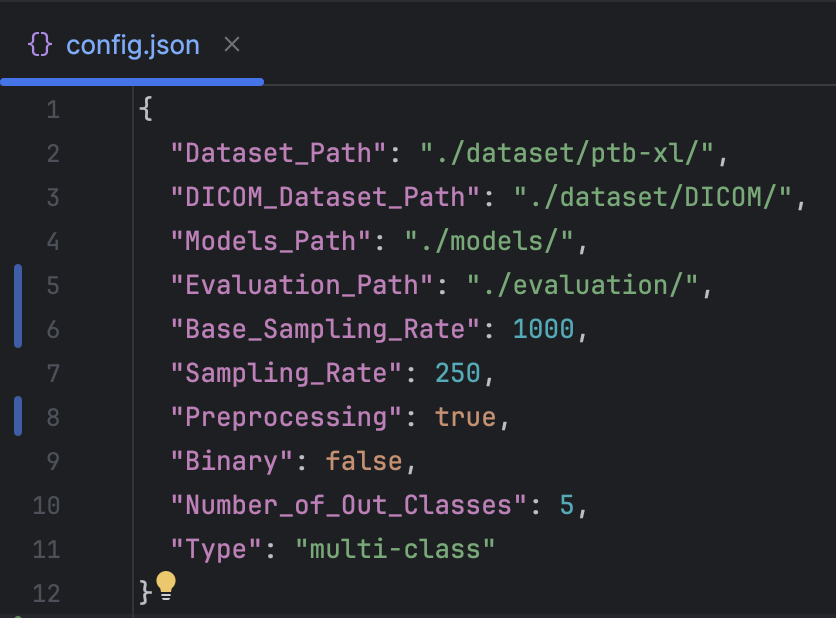
\includegraphics[alt={Cattura dello schermo rappresentante il \textit{file} di \textit{config}}, width=0.8\columnwidth]{img/config.png}
    \caption{\centering Cattura dello schermo rappresentante il \textit{file} di \textit{config}}
    \label{fig:config}
\end{figure}\noindent
A fine dell'esecuzione del programma, l'utente può trovare le varie valutazioni all'interno di una cartella specifica contenuta nella \textit{directory} del progetto. Di seguito mostro un'esempio dei contenuti prodotti:
\begin{figure}[H]
    \centering
    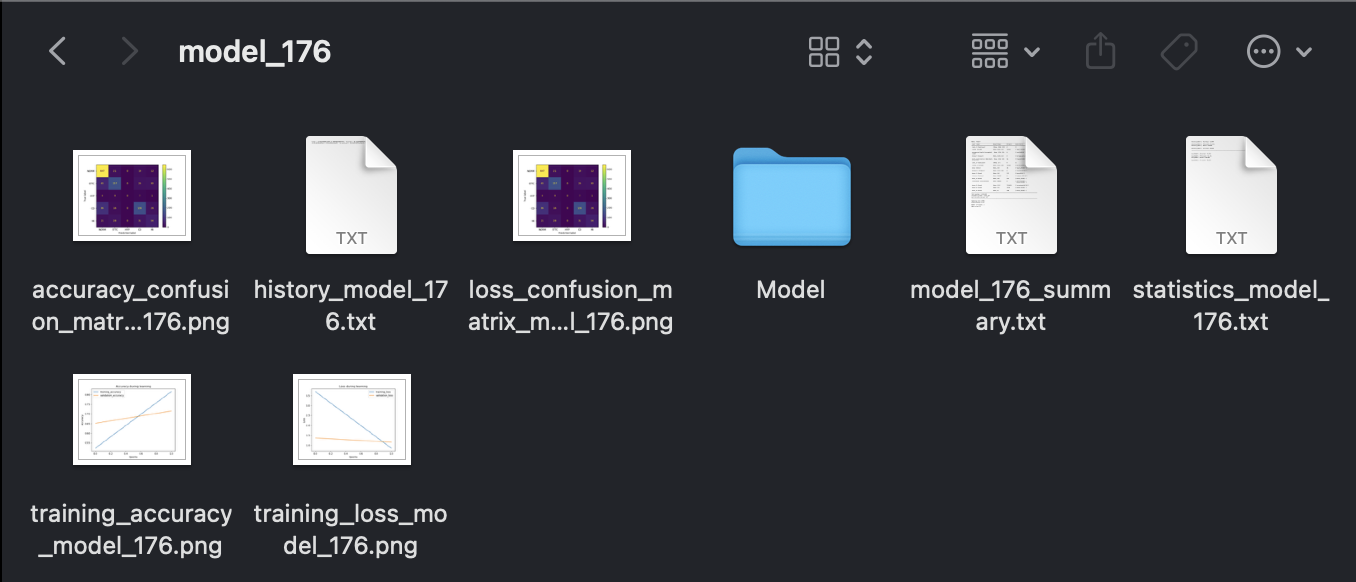
\includegraphics[alt={Cattura dello schermo rappresentante i \textit{file} di \textit{output}}, width=0.9\columnwidth]{img/output.png}
    \caption{\centering Cattura dello schermo rappresentante i \textit{file} di \textit{output}}
    \label{fig:output}
\end{figure}\noindent
Inoltre, durante allo \textit{stage} avevo l'obiettivo di realizzare io stesso dei \textit{training} di reti neurali artificiali.
Perciò ho anche prodotto due modelli cercando di ottenere delle buone prestazioni. Essi sono due perchè ho salvato solo i risultati migliori che ho ottenuto per due tipi di classificazione: binaria, ovvero sano o non sano, e multi-classe, dove il modello predice il risultato su cinque possibili classi.

\subsection{Piano quantitativo}\noindent
% \texttt{Esposizione dei risultati ottenuti sul piano quantitativo, qui vengono illustrate la copertura dei requisiti e dei test.}
Sul piano quantitativo sono riuscito a soddisfare tutti i requisiti derivanti dall'analisi dei requisiti e rappresentati nella tabella \ref{tab:user-stories}.\\
Per quanto riguarda il \textit{code coverage}, non avendo creato solo test automatici, ma svolto test manuali per via della natura del progetto: non posso quantificare in modo obiettivo questa metrica.\\
Tuttavia posso parlare dei risultati ottenuti con l'attività di addestramento.
\begin{center}
    \rowcolors{1}{}{tableGray}
    \begin{longtable}{|p{2.5cm}|p{2.5cm}|}
    \hline
    \multicolumn{2}{|c|}{\textbf{\textit{Binary model}}} \\ 
    \hline 
    \endfirsthead
    \rowcolor{white}
    \multicolumn{2}{c}{{\bfseries \tablename\ \thetable{} -- Continuo della tabella}}\\
    \hline
    \multicolumn{1}{|c|}{\textbf{Identificatore}} & \multicolumn{1}{c|}{\textbf{\textit{User story}}}\\ \hline 
    \endhead
    \hline
    \rowcolor{white}
    \multicolumn{2}{|r|}{{Continua nella prossima pagina...}}\\
    \hline
    \endfoot
    \endlastfoot
    
    \multicolumn{1}{|c|}{\textit{Accuracy}} & \multicolumn{1}{|c|}{86.25\%} \\
    \hline
    \multicolumn{1}{|c|}{\textit{Precision}} & \multicolumn{1}{|c|}{87.93\%} \\
    \hline
    \multicolumn{1}{|c|}{\textit{Recall}} & \multicolumn{1}{|c|}{81.07\%} \\
    \hline
    \multicolumn{1}{|c|}{\textit{Specificity}} & \multicolumn{1}{|c|}{90.63\%} \\
    \hline
    \multicolumn{1}{|c|}{\textit{F1 Score}} & \multicolumn{1}{|c|}{84.36\%} \\
    \hline
    \hiderowcolors
    \caption{Tabella contenente le prestazioni del modello binario.}
    \label{tab:bin-model-res}
    \end{longtable}

    \rowcolors{1}{}{tableGray}
    \begin{longtable}{|p{2.5cm}|p{2.5cm}|}
    \hline
    \multicolumn{2}{|c|}{\textbf{\textit{Multi-class model}}} \\ 
    \hline 
    \endfirsthead
    \rowcolor{white}
    \multicolumn{2}{c}{{\bfseries \tablename\ \thetable{} -- Continuo della tabella}}\\
    \hline
    \multicolumn{1}{|c|}{\textbf{Identificatore}} & \multicolumn{1}{c|}{\textbf{\textit{User story}}}\\ \hline 
    \endhead
    \hline
    \rowcolor{white}
    \multicolumn{2}{|r|}{{Continua nella prossima pagina...}}\\
    \hline
    \endfoot
    \endlastfoot
    
    \multicolumn{1}{|c|}{\textit{Accuracy}} & \multicolumn{1}{|c|}{71.50\%} \\
    \hline
    \multicolumn{1}{|c|}{\textit{Precision}} & \multicolumn{1}{|c|}{51.11\%} \\
    \hline
    \multicolumn{1}{|c|}{\textit{Recall}} & \multicolumn{1}{|c|}{48.85\%} \\
    \hline
    \multicolumn{1}{|c|}{\textit{F1 Score}} & \multicolumn{1}{|c|}{49.65\%} \\
    \hline
    \hiderowcolors
    \caption{Tabella contenente le prestazioni del modello multi-classe.}
    \label{tab:multiclass-model-res}
    \end{longtable}
\end{center}\noindent
Come si può vedere nelle tabelle \ref{tab:bin-model-res} e \ref{tab:multiclass-model-res}, i modelli creati da me non sono veramente ottimi, sopratutto se vengono seguiti gli \textit{standard} richiesti in campo medico, dove si richiede un'accuratezza più alta possibile.\\
Tuttavia, questi risultati non sono causati da mie scelte errate di configurazione, ma al \textit{dataset} utilizzato.
Avendo utilizzato per la maggior parte il \textit{dataset} pubblico PTB-XL di PhysioNet, ho potuto confrontare i miei risultati ottenuti con una ricerca scientifica che ha svolto i miei stessi tipi di addestramenti di reti neurali artificiali.\\
La pubblicazione scientifica in questione è \citetitle{article:ecg-paper}, dove vengono mostrati dei risultati finali simili a quello che ho ottenuto, solo marginalmente migliori.